\bab{BAB III}{METODE PENELITIAN}


% \addcontentsline{toc}{chapter}{BAB II TINJAUAN PUSTAKA}
\setcounter{chapter}{3}
\setcounter{section}{0} % RESET section ke 0
\renewcommand{\thesection}{\thechapter.\arabic{section}}
Penelitian ini menggunakan metode \parencite{santoso2020implementasi} dalam bentuk eksperimen untuk mengevaluasi model deep learning dalam tugas prediksi waypoint, segmentasi semantik, dan ekstraksi fitur visual pada sistem kendaraan otonom. Pada Gambar \ref{fig:desain_penelitian} dapat dilihat desain penelitian yang digunakan dalam penelitian ini. Penelitian ini bermulai dari  perumusan masalah, kemudian dilanjutkan dengan studi literatur, pengumpulan data, praproses data, perancangan algoritma, pelatihan model, evaluasi model, dan terakhir penarikan kesimpulan.
\vspace{1cm}
\begin{figure}[H]
    \centering
    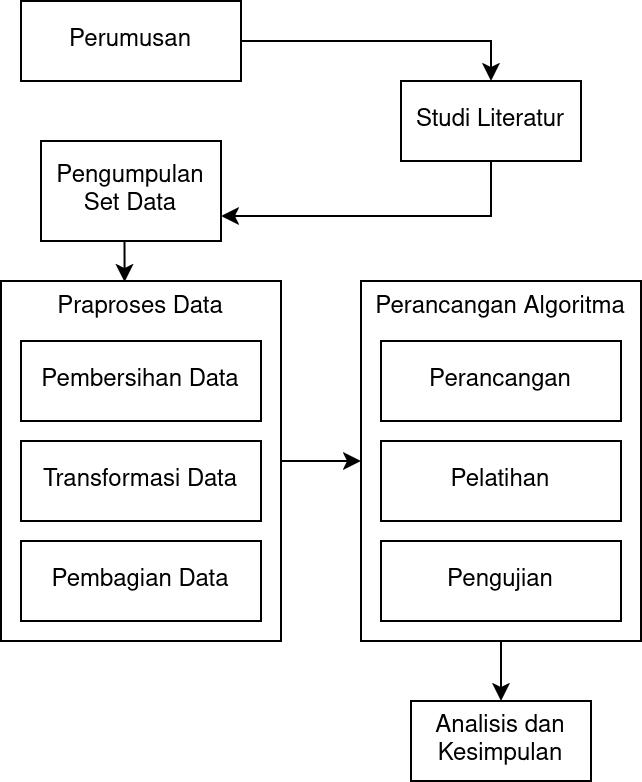
\includegraphics[width=0.6\textwidth]{images/desain-penelitian.png}
    \caption{Desain Penelitian.}
    \label{fig:desain_penelitian}
\end{figure}

\section{Pengumpulan Set Data}

\subsection{Variasi Dataset}
\begin{equation}
    D = \{(X_i, Y_i)\}_{i=1}^{J}
\end{equation}


\subsection{Representasi Data}
\begin{enumerate}
    \item{LiDAR Point Clouds}\\
    Lidar point clouds direpresentasikan sebagai tensor 3D dengan dimensi pada
$
    \mathbb{R}^{4 \times 13716}
$
di mana 4 adalah jumlah fitur (x, y, z, intensitas) dan 13716 adalah jumlah titik yang diambil dari LiDAR. Data point cloud ini memberikan informasi tentang posisi dan intensitas cahaya yang dipantulkan oleh objek di sekitar kendaraan.


    \item{Segmentasi Semantik}\\
\begin{equation}
    R \in \{0, 1\}^{23 \times 256 \times 256}
\end{equation},
    \item{Waypoints}\\
Waypoints dilambangkan sebagai
\begin{equation}
    \omega_i^\rho = (x_i, y_i)
\end{equation}

    \item{Kontrol Kendaraan}\\
    \label{sec:kontrol_kendaraan}

Steering $\in [-1, 1]$

Throttle $\in [0, 0.75]$

Brake $\in [0, 1]$


    \item{Informasi Tambahan}\\
\end{enumerate}


\subsection{Konfigurasi Data CARLA}


\begin{table}[H]
\centering
\caption{Carla Dataset Setting}
\label{tab:carla_dataset_setting}
\begin{tabularx}{\textwidth}{lX}
\hline
\textbf{Maps} & Town01, Town02, Town03, Town04, Town05, Town06, Town07, Town10 \\
\hline
\textbf{Route sets*} & 
Long (1000--200m), Short (100--500m), Tiny (one turn or one go-straight) \\
\hline
\textbf{Weather presets} & ClearNoon \\
\hline
\textbf{Non-playable characters} & Vehicles (truck, car, bicycle, motorbike) and pedestrians \\
\hline
\textbf{Object classes} & 
0: Unlabeled, 1: Building, 2: Fence, 3: Other, 4: Pedestrian, 5: Pole, 6: Road lane, 7: Road, 8: Sidewalk, 9: Vegetation, 10: Other vehicles, 11: Wall, 12: Traffic sign, 13: Sky, 14: Ground, 15: Bridge, 16: Rail track, 17: Guard Trail, 18: Traffic light, 19: Static Object, 20: Dynamic Object, 21: Water, 22: Terrain \\
\hline
\textbf{CARLA version} & 0.9.10.1 \\
\hline
\end{tabularx}
\end{table}
\section{Praproses Data}
\subsection{Pembersihan Data}
\subsection{Transformasi Data}

        Formula yang digunakan untuk mendekode nilai kedalaman adalah sebagai berikut \parencite{carladepthcamera}:
        \begin{equation}
            \mathbb{R}_i^{\text{dec}} = \frac{R_i + 256 G_i + 256^2 B_i}{256^3 - 1} \times 1000,
            \end{equation}
      

\subsubsection{Swin Transformer Varians}
Swin Transformer memiliki beberapa varian yang berbeda, masing-masing dengan karakteristik dan ukuran yang berbeda. Tabel \ref{tab:swin_variants} menunjukkan perbandingan antara varian-varian tersebut, termasuk ukuran patch, dimensi embedding, jumlah layer, jumlah head, jumlah parameter (M), dan FLOPs (G). Setiap varian memiliki keunggulan dan kelemahan masing-masing, sehingga pemilihan varian yang tepat sangat penting untuk mencapai performa yang optimal dalam tugas-tugas tertentu.
\begin{table}[H]
    \centering
    \caption{Varian Swin Transformer dan Karakteristiknya}\label{tab:swin_variants}
    \resizebox{\textwidth}{!}{%
    \begin{tabular}{lccccccp{5cm}}
    \hline
    \textbf{Varian} & \textbf{Patch Size} & \textbf{Dimensi Embed} & \textbf{Jumlah Layer} & \textbf{Jumlah Head} & \textbf{Param (M)} & \textbf{FLOPs (G) @224} & \textbf{Ciri Khas} \\
    \hline
    Swin-T (Tiny)  & 4×4 & 96  & [2, 2, 6, 2]  & [3, 6, 12, 24]  & 28M  & 4.5  & Ringan, cocok untuk device terbatas \\
    Swin-S (Small) & 4×4 & 96  & [2, 2, 18, 2] & [3, 6, 12, 24]  & 50M  & 8.7  & Trade-off antara performa dan ukuran \\
    Swin-B (Base)  & 4×4 & 128 & [2, 2, 18, 2] & [4, 8, 16, 32]  & 88M  & 15.4 & Performansi tinggi, sering dipakai \\
    Swin-L (Large) & 4×4 & 192 & [2, 2, 18, 2] & [6, 12, 24, 48] & 197M & 34.5 & Sangat kuat, untuk tugas kompleks \\
    \hline
    \end{tabular}%
    }
    \end{table}
    


\subsection{Evaluasi}